\documentclass[11pt]{article}

% ---- Swap this preamble block for a venue style (neurips/icml/acl) at submission. ----
\usepackage[margin=1in]{geometry}
\usepackage{graphicx}
\usepackage{booktabs}
\usepackage{amsmath,amssymb}
\usepackage{siunitx}
\usepackage[numbers,round]{natbib}
\usepackage[hidelinks]{hyperref}
\usepackage{xcolor}
\usepackage{caption}
\captionsetup{font=small,labelfont=bf}
\graphicspath{{figures/}}

\title{Routed Experts Are Not Redundant: The Shared-Expert\\ Gradient Race in Small Mixture-of-Experts Models}
\author{TBD}
\date{}

\begin{document}
\maketitle

\begin{abstract}
Small Mixture-of-Experts (MoE) language models with a DeepSeek-style shared expert are a popular
testbed for interpretability, because they are cheap to train and every token can be labelled. A
recurring observation in this regime is that the routed experts appear \emph{redundant}: ablating
the entire routed branch barely changes perplexity, while the single always-on shared expert
dominates the feed-forward computation. We show that this ``routed redundancy'' is largely an
\textbf{artifact of undertraining}, and we identify its cause. Using a 134M-parameter MoE trained
from scratch on a three-domain, token-labelled corpus, we find that (i) the shared expert carries
$\sim$80\% of the feed-forward ablation impact at 98M tokens but the routed and shared branches
become \textbf{balanced by $\sim$300M tokens} and stay balanced through 1B (4 seeds, tight error
bars); (ii) this early dominance is a \textbf{gradient-exposure race}---the shared expert receives
gradient from 100\% of tokens versus $\sim\!k/E$ per routed expert, so it wins the early
optimization race; and (iii) the race is \textbf{causally controllable}: slowing the shared
expert's learning rate shifts the routed-activation crossover dose-dependently (the shared
branch's share of ablation impact at 98M tokens drops from 0.80 to 0.14) \textbf{at no perplexity
cost}. A single hyperparameter thus reallocates computation to the routed experts without changing
model quality. The control \textbf{reproduces at $2\times$ depth}, and a \emph{temporary} handicap
suffices: once the shared expert's learning rate is ramped back to parity, the reallocation
persists to 1B tokens. Finally we identify what sets \emph{where} the split lands---not the number
of experts, but the \textbf{routed:shared width ratio}. Holding the routed branch byte-for-byte
identical and varying only the shared expert's width moves the shared branch's share from 0.28 to
0.81, and the ratio orders every configuration we measured across $8\times$ in ratio, $8\times$ in
expert count and $4\times$ in parameter count. We further report the axes of specialization
(surface form $>$ domain $>$ frequency, position irrelevant). Three of our own conclusions were
overturned by seed replication or better controls and are reported as such.
\end{abstract}

\section{Introduction}

Mixture-of-Experts layers replace a dense feed-forward block with a router that dispatches each
token to a small number of experts. The DeepSeekMoE design~\citep{dai2024deepseekmoe} adds an
always-on \emph{shared expert} alongside the \emph{routed} experts, on the intuition that the
shared expert absorbs common computation and frees the routed experts to specialize. Because small
MoEs are cheap and controllable, they are widely used to study expert specialization.

In this small-scale regime, a striking and repeatedly observed phenomenon is that the routed
experts look nearly useless: removing all of them costs little perplexity, while removing the lone
shared expert costs a lot. It is tempting to conclude that small MoEs are over-parametrized on the
routed side, or that the shared expert suppresses the routed experts.

We show that this conclusion is \textbf{premature}. The apparent redundancy is a transient property
of early training that disappears with enough tokens, and its cause is a simple, controllable
optimization dynamic. Our contributions:
\begin{enumerate}
  \item \textbf{Observation.} Branch importance is a function of tokens seen: routed ``redundancy''
  and shared dominance vanish by $\sim$300M tokens (Section~\ref{sec:obs}).
  \item \textbf{Mechanism.} The dominance is a \emph{gradient-exposure race}---the shared expert is
  updated on every token, each routed expert on a $k/E$ fraction---proven causally by slowing the
  shared expert and watching the crossover shift, at no quality cost (Section~\ref{sec:mech}).
  \item \textbf{Control.} One hyperparameter (shared-expert learning rate) sets when---and
  whether---the routed experts engage, and a \emph{temporary} handicap is enough: the reallocation
  persists after the handicap is lifted (Section~\ref{sec:mech}).
  \item \textbf{What sets the split.} Where the two branches settle is governed by the
  routed:shared \emph{width ratio}, not by the number of experts; this supersedes an earlier
  non-monotonic \#experts result of ours, confounded by total routed capacity
  (Section~\ref{sec:scope}).
\end{enumerate}
Along the way we characterize \emph{what} the experts specialize by, and we explicitly retract
three earlier findings that did not survive replication or better controls
(Section~\ref{sec:support}). We view the honest,
seed-replicated, causal methodology as part of the contribution.

\section{Related work}

\paragraph{Sparse MoE layers.} Conditional computation via a sparsely-gated MoE layer was
introduced by \citet{shazeer2017outrageously} and scaled by GShard~\citep{lepikhin2021gshard} and
Switch Transformer~\citep{fedus2022switch}, which also established the auxiliary load-balancing
loss. ST-MoE~\citep{zoph2022stmoe} added the router z-loss for stability. Our model uses both, in a
top-2 configuration~\citep{jiang2024mixtral}.

\paragraph{Shared experts.} DeepSeekMoE~\citep{dai2024deepseekmoe} introduced the always-on shared
expert alongside fine-grained routed experts, arguing it absorbs common knowledge and thereby
\emph{frees} the routed experts to specialize; the design carries through
DeepSeek-V2/V3~\citep{deepseekv2,deepseekv3}, which also motivate auxiliary-loss-free routing by the
balance--specialization tension. We reproduce the ``shared enables specialization'' effect
(Section~\ref{sec:support}) but show it is only visible once balancing is off, and---more
importantly---that at small scale the shared expert \emph{dominates} the computation for a
mechanistic reason unrelated to specialization.

\paragraph{Expert specialization studies.} Analyses of Mixtral~\citep{jiang2024mixtral} report that
experts specialize more by token/syntactic identity than by topic; OLMoE~\citep{muennighoff2024olmoe}
studies specialization and routing across training in open MoEs. We add a controlled,
domain-labelled probe with causal branch ablation and, crucially, identify a training-dynamics cause
for the small-scale ``routed redundancy'' that these observational studies do not address.

\paragraph{Architecture components.} Our backbone uses MLA~\citep{deepseekv2}, RoPE~\citep{su2021roformer},
RMSNorm~\citep{zhang2019rmsnorm}, and optional YaRN context extension~\citep{peng2023yarn}; the
distillation experiment follows \citet{hinton2015distilling} with a Mistral-7B
teacher~\citep{jiang2023mistral}. Pre-training data are FineWeb-Edu~\citep{penedo2024fineweb},
Cosmopedia-v2~\citep{benallal2024cosmopedia}, and OpenWebMath~\citep{paster2023openwebmath}.

To our knowledge, the central claim---that small-MoE routed redundancy is an \emph{undertraining
artifact} caused by a \emph{gradient-exposure race} between the shared and routed experts, and is
\emph{causally controllable} by the shared-expert learning rate at no quality cost---is new.

\section{Setup}\label{sec:setup}

\paragraph{Model.} A decoder-only MoE re-implemented from scratch in PyTorch: Multi-head Latent
Attention (MLA), RoPE, RMSNorm, and per layer a MoE block with 8 routed experts $+$ 1 shared
expert and top-2 routing (134M parameters, 8 layers, hidden 512, context 512). Every expert, routed
or shared, has intermediate width 1024 unless stated otherwise; Section~\ref{sec:scope} varies the
two widths independently and writes them $I$ (per routed expert) and $I_{\mathrm{shared}}$. During
analysis we run the MoE in inference mode (no capacity dropping), which we verified is numerically
identical to the training MoE when no tokens are dropped.

\paragraph{Data.} Pre-training streams three token-labelled corpora: FineWeb-Edu (\texttt{web},
60\%), Cosmopedia-v2 (\texttt{edu}, 25\%), OpenWebMath (\texttt{math}, 15\%), tokenized with the
Mistral vocabulary (32k). Sequences are packed to 512 tokens. The domain labels are the key lever:
they let us attribute routing to a known variable. Held-out per-domain evaluation packs each domain
separately (one label per sequence).

\paragraph{Metrics.} \emph{Branch importance}: $\Delta$PPL from ablating a whole branch (all routed
experts, or the shared expert). This whole-branch ablation is the correct causal probe---single-expert
ablation is misleading because top-2 routing reroutes to the survivors. The \emph{shared share} is
$\Delta_{\text{shared}}/(\Delta_{\text{shared}}+\Delta_{\text{routed}})$. \emph{Specialization}:
gate-weighted normalized mutual information $\mathrm{NMI}(\text{Expert};\text{axis})=I/H$, averaged
over layers, against a label-permutation null ($\approx 0$ everywhere). \emph{Balance}: std of top-1
expert load. Between-condition tests are exact permutation tests on seed-level values (minimum
two-sided $p=2/\binom{2n}{n}$ for $n$ seeds per group).

\paragraph{Compute.} All runs are on one NVIDIA RTX A6000 using a plain single-GPU trainer; the
largest models see $\sim$1B tokens ($\sim$3.4h each).

\section{Routed ``redundancy'' is an undertraining artifact}\label{sec:obs}

We train the base model for 30k steps ($\sim$983M tokens, batch 64), 4 seeds, and measure branch
importance at each checkpoint (mean $\pm$ std, Table~\ref{tab:f8}, Figure~\ref{fig:f8}).

\begin{table}[t]
\centering
\caption{Branch importance vs.\ tokens (baseline, 4 seeds, batch 64).}
\label{tab:f8}
\begin{tabular}{rrrrrr}
\toprule
tokens & PPL & remove shared & remove all routed & routed NMI & shared share \\
\midrule
98M  & 4.18 & $+3.44\pm0.17$ & $+0.82\pm0.03$ & 0.0121 & 0.81 \\
197M & 3.63 & $+2.37\pm0.17$ & $+1.58\pm0.06$ & 0.0148 & 0.60 \\
295M & 3.41 & $+1.99\pm0.14$ & $+1.98\pm0.06$ & 0.0161 & 0.50 \\
491M & 3.20 & $+1.99\pm0.16$ & $+2.25\pm0.01$ & 0.0168 & 0.47 \\
983M & 3.00 & $+2.45\pm0.18$ & $+2.48\pm0.11$ & 0.0174 & 0.50 \\
\bottomrule
\end{tabular}
\end{table}

\begin{figure}[t]
\centering
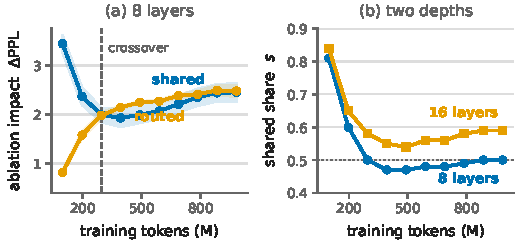
\includegraphics[width=0.72\linewidth]{fig1_trajectory.pdf}
\caption{Ablation impact ($\Delta$PPL) of removing the shared expert vs.\ all 8 routed experts,
over a 4-seed constant-batch trajectory (bands $=\pm1$ std). The shared expert dominates early;
the branches cross to balance by $\sim$295M tokens.}
\label{fig:f8}
\end{figure}

At 98M tokens---the regime of many pilot studies and of our own early experiments---the shared
expert carries 81\% of the ablation impact and the routed experts look nearly redundant. The
crossover to balance happens by $\sim$295M tokens, after which the branches contribute equally
through 1B. All four seeds follow the same trajectory with tight error bars; routed specialization
grows in parallel (NMI $0.0008\rightarrow0.017$). \textbf{Conclusions drawn about routed redundancy
or shared dominance below a few hundred million tokens do not generalize.}

\section{The mechanism: a gradient-exposure race}\label{sec:mech}

Why does the shared expert dominate early? It is updated on \textbf{every} token; each routed
expert is updated on only a $k/E = 2/8 = 25\%$ fraction. The shared expert therefore wins the early
optimization race and the residual stream comes to rely on it; the routed experts become
load-bearing only once the shared expert saturates.

\paragraph{Formalization.} Consider one MoE block whose output on token $t$ is
\begin{equation}
y_t = s(x_t) + \sum_{e\in\mathrm{topk}(t)} g_{t,e}\, f_e(x_t),
\end{equation}
where $s$ is the shared expert and $f_e$ the routed experts. Over a batch of $N$ tokens, the shared
parameters receive gradient aggregated over all $N$ tokens, whereas a routed expert $e$ receives
gradient only from the $\approx N k/E$ tokens routed to it. Under a shared learning rate, the shared
expert accumulates roughly $E/k\times$ more effective updates per parameter early in training, when
the loss gradient is large and the allocation of ``who computes what'' is still plastic. The
residual pathway greedily routes common computation to whichever sub-module reduces loss
fastest---the shared expert---further starving the routed experts (a rich-get-richer dynamic). This
yields two testable predictions: (i) reducing the shared expert's learning rate should let the
routed experts capture computation earlier (confirmed below); and (ii) the crossover token count
should grow with $E/k$ (Section~\ref{sec:scope}, \textbf{refuted}---expert count barely moves the
split; the relative \emph{width} of the two branches is what governs it).

We test prediction (i) by placing the shared-expert parameters in their own optimizer group at
$\mathrm{lr}\times\text{mult}$, everything else at the base learning rate (2 seeds; values at 98M
tokens, Table~\ref{tab:f9}, Figure~\ref{fig:f9}).

\begin{table}[t]
\centering
\caption{Shared-expert LR sweep (2 seeds), at 98M tokens.}
\label{tab:f9}
\begin{tabular}{lrrrr}
\toprule
shared LR & remove routed & remove shared & shared share & PPL \\
\midrule
$\times1.0$ (baseline) & $+0.85$ & $+3.46$ & 0.80 & 4.16 \\
$\times0.3$ & $+1.94$ & $+2.48$ & 0.56 & 4.10 \\
$\times0.1$ & $+4.46$ & $+0.72$ & 0.14 & 4.10 \\
\bottomrule
\end{tabular}
\end{table}

\begin{figure}[t]
\centering
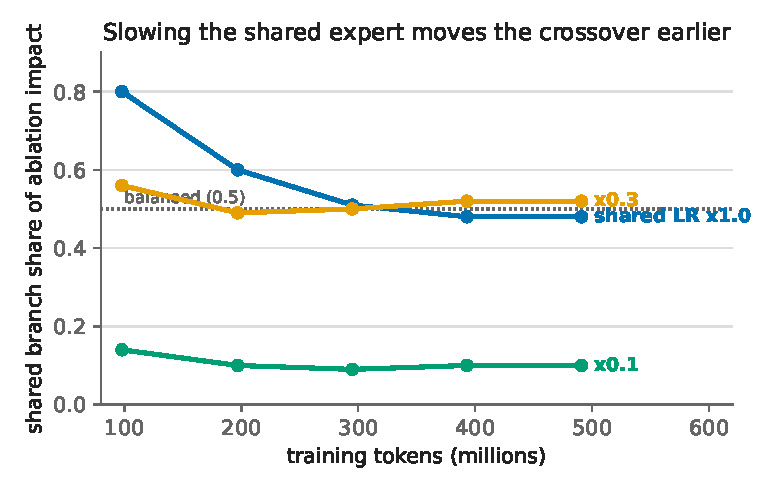
\includegraphics[width=0.72\linewidth]{fig2_mechanism.pdf}
\caption{Shared branch's share of ablation impact vs.\ tokens, for three shared-expert
learning-rate multipliers (2 seeds). Slowing the shared expert shifts the routed-activation
crossover earlier, dose-dependently---at unchanged perplexity.}
\label{fig:f9}
\end{figure}

Slowing the shared expert makes the routed branch load-bearing \textbf{dramatically earlier}---a
$5\times$ increase in routed importance at a \emph{fixed} token budget---shifting the crossover from
$\sim$295M tokens (baseline) to $<$100M ($\times0.3$) to before training even settles ($\times0.1$,
where routed dominate from the start). The effect is monotonic, dose-dependent, tight error bars.
This \textbf{refutes autonomous routed maturation}: the routed experts were being out-competed, not
merely immature. Crucially, \textbf{held-out perplexity is unchanged} across conditions. The shared
expert is therefore not \emph{necessary} for this computation; the model defaults to placing it
there because that expert trains fastest. A single knob reallocates computation to the routed
experts at no quality cost.

\paragraph{Does the mechanism hold at scale?} We repeat the shared-LR sweep on a $2\times$-deeper
model (16 layers, 251M parameters, 1 seed; Figure~\ref{fig:scale}). The control reproduces almost
exactly: at 98M tokens the shared share drops $0.82\rightarrow0.64\rightarrow0.21$ for
$\times1.0/\times0.3/\times0.1$ (vs.\ $0.80/0.56/0.14$ at 134M), dose-dependent and at unchanged
perplexity---the gradient-race mechanism and its knob are robust to depth. The crossover
\emph{timing}, however, is scale-dependent: the deeper baseline only reaches a minimum share of
$0.54$ ($\sim$491M tokens) and does \textbf{not} cross to balance within 1B tokens, the shared
expert re-asserting dominance ($0.59$ at 983M). This dip-then-rise shape is universal in our runs:
every configuration in Section~\ref{sec:scope} shows it, at a level set by the width ratio, which
is why we report the minimum over the trajectory there rather than the endpoint. Deeper models stay
shared-dominated for many more tokens; ``enough tokens'' for routed balance grows with model size
(mechanistically consistent). This strengthens the practical warning but means that \emph{left
alone} we observe the crossover complete only at our smallest configuration within our 1B-token
budget. The next experiment shows the deeper model can nonetheless be driven past balance and kept
there.

\begin{figure}[t]
\centering
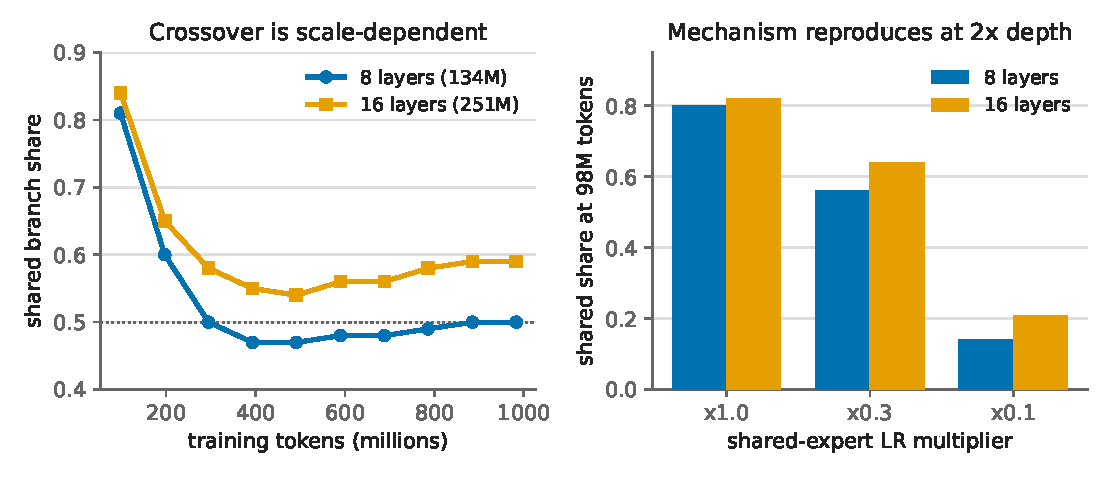
\includegraphics[width=0.92\linewidth]{fig5_scale.pdf}
\caption{(left) shared branch's share vs.\ tokens at two depths---the 8-layer model crosses to
balance, the 16-layer model approaches but does not within 1B tokens; (right) the shared-LR
control reproduces at $2\times$ depth, dropping the share dose-dependently at both scales.}
\label{fig:scale}
\end{figure}

\paragraph{A temporary handicap is enough.} If the split is decided by an early race, handicapping
the shared expert only \emph{during} that race should suffice. We ramp the shared-expert LR
multiplier from $\times0.1$ up to $\times1.0$ by step 9000 ($\sim$295M tokens) on the 16-layer model
(251M parameters, 1 seed), after which every parameter trains at the base rate
(Table~\ref{tab:hyst}, Figure~\ref{fig:hyst}). The reallocation \textbf{does not undo}: by the end
of the ramp the ramped run has converged onto the static-$\times0.1$ trajectory, and once the
handicap is gone it stays there---$0.21$ at 983M tokens versus the baseline's $0.59$, at equal
perplexity (2.89 vs.\ 2.90). The shared branch re-asserts only slowly ($0.14\rightarrow0.21$ between
295M and 983M), far more slowly than the baseline's rise. This is what a race-then-commit dynamic
predicts, and it makes the knob a \emph{training-schedule} intervention rather than a permanent tax
on the shared expert. It is, however, a single seed at one ramp endpoint and one depth; we claim
existence, not a law.

\begin{table}[t]
\centering
\caption{Shared branch share vs.\ tokens at 16 layers (251M), for a constant, a static and a ramped
shared-expert learning rate. The static $\times0.1$ run stopped at 491M tokens.}
\label{tab:hyst}
\begin{tabular}{lrrr}
\toprule
tokens & baseline $\times1.0$ & static $\times0.1$ & ramp $0.1\rightarrow1.0$ \\
\midrule
98M                 & 0.84 & 0.21 & 0.42 \\
295M (ramp ends)    & 0.58 & 0.14 & 0.15 \\
491M                & 0.54 & 0.16 & 0.16 \\
983M                & 0.59 & ---  & \textbf{0.21} \\
\midrule
final PPL           & 2.90 & ---  & 2.89 \\
\bottomrule
\end{tabular}
\end{table}

\begin{figure}[t]
\centering
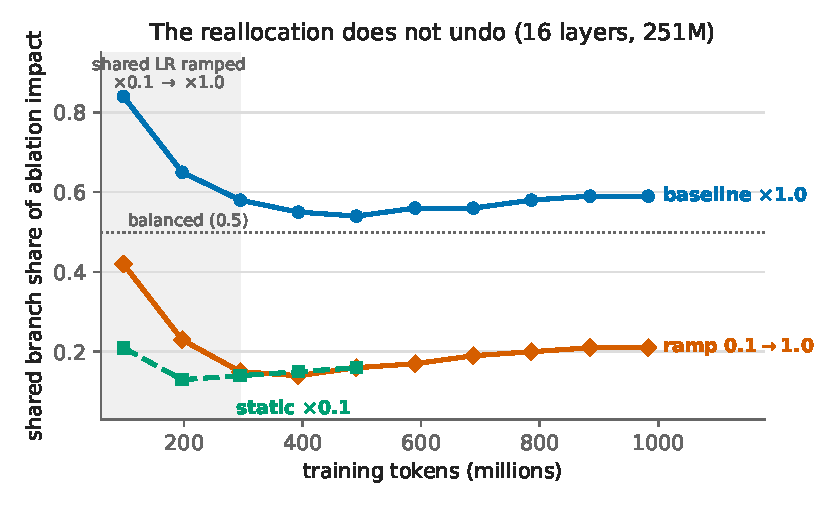
\includegraphics[width=0.72\linewidth]{fig6_hysteresis.pdf}
\caption{Ramping the shared-expert learning rate back to parity by 295M tokens (shaded) leaves the
reallocation essentially in place through 1B tokens, rather than returning to the baseline
trajectory. 16 layers, 251M parameters, 1 seed.}
\label{fig:hyst}
\end{figure}

\section{What sets the split: the routed:shared width ratio}\label{sec:scope}

Section~\ref{sec:mech} explains \emph{why} the shared expert wins early and shows the race can be
rigged; it does not say where the split finally lands. The gradient-race picture naively predicts
that quantity should be governed by $E/k$. We tested that across eleven 8-layer configurations
(top-2, 983M tokens, 1--2 seeds each; seven run specifically for this section), and the prediction
fails: expert count barely matters, while the \textbf{ratio of the two branches' widths} orders
every run we measured.

Two contrasts disentangle the candidates (Table~\ref{tab:ratio}). Both hold $E{=}8$ and $k{=}2$
fixed, so expert count, routing and per-expert gradient share are constant throughout. The second
is the decisive one: with $I$ pinned at 1024 the routed branch is byte-for-byte identical across
the three runs---same expert count, same per-expert width, same active capacity $k\cdot I = 2048$
---and the split still moves by 0.53. \textbf{Absolute routed capacity therefore does not govern
the split.}

\begin{table}[t]
\centering
\caption{The two disentangling contrasts, both at $E{=}8$, $k{=}2$. Values are the minimum shared
share reached over the trajectory.}
\label{tab:ratio}
\begin{tabular}{lrrr}
\toprule
\multicolumn{4}{l}{\emph{Varying routed width} ($I_{\mathrm{shared}} = 1024$)}\\
$I$              & 256    & 1024   & 2048 \\
min shared share & 0.79   & 0.47   & 0.37 \\
params           & 58.2M  & 133.7M & 234.4M \\
\midrule
\multicolumn{4}{l}{\emph{Varying shared width} ($I = 1024$; routed branch identical)}\\
$I_{\mathrm{shared}}$ & 512   & 1024   & 4096 \\
min shared share  & \textbf{0.28} & 0.47 & \textbf{0.81} \\
params            & 127.4M & 133.7M & 171.5M \\
\bottomrule
\end{tabular}
\end{table}

What the two contrasts have in common is the ratio $I/I_{\mathrm{shared}}$. Grouping every
configuration by it---including the four points of our earlier \#experts sweep, all of which sat
at ratio 1.0---gives non-overlapping bands (Figure~\ref{fig:f10}):

\begin{center}
\begin{tabular}{lcccc}
\toprule
ratio $I/I_{\mathrm{shared}}$ & 0.25 & 0.5 & 1.0 & 2.0 \\
\midrule
min shared share & 0.72 / 0.79 / 0.81 & 0.63 & 0.47 / 0.53 / 0.55 / 0.56 & 0.25 / 0.28 / 0.37 \\
\bottomrule
\end{tabular}
\end{center}

\begin{figure}[t]
\centering
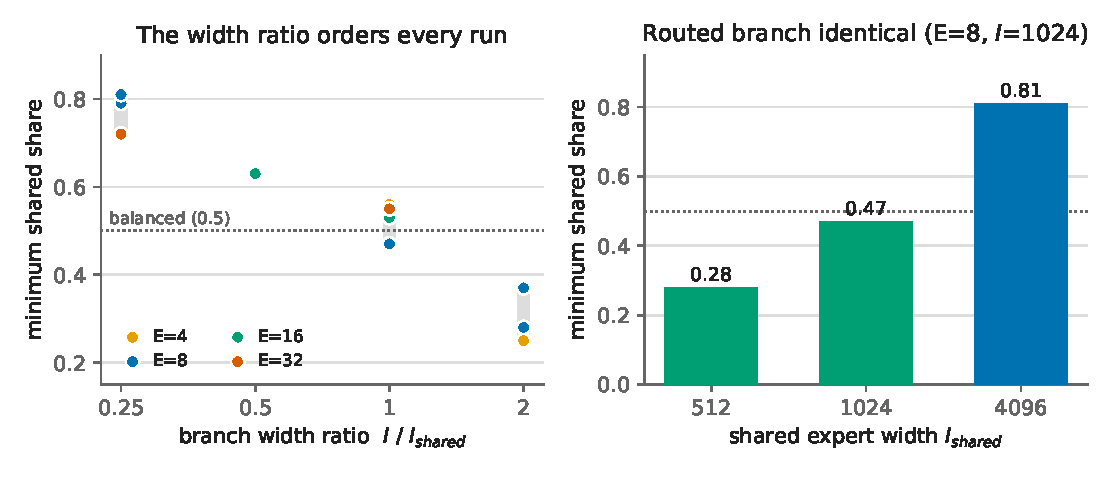
\includegraphics[width=0.92\linewidth]{fig3_ratio.pdf}
\caption{(left) minimum shared share vs.\ the branch width ratio, one point per configuration,
coloured by expert count; the bands per ratio level do not overlap. (right) the decisive
contrast---the routed branch is identical in all three runs and only the shared expert's width
changes.}
\label{fig:f10}
\end{figure}

The ordering holds across $8\times$ in ratio, $8\times$ in expert count ($E\in\{4,\dots,32\}$) and
$4\times$ in parameter count (58M--234M). Within a band the residual spread is $\sim$0.1 and is
\textbf{not} consistently explained by $E$: at ratio 2.0 more experts \emph{raise} the share
($E{=}4\rightarrow0.25$ vs.\ $E{=}8\rightarrow0.37$) while at ratio 0.25 more experts \emph{lower}
it ($E{=}32\rightarrow0.72$ vs.\ $E{=}8\rightarrow0.79$). Seed noise on this quantity is
$\sim$0.02, an order of magnitude below the effect. Holding total routed capacity fixed instead
($E\cdot I = 8192$ at equal parameters) leaves perplexity flat as well---2.99 / 3.00 / 3.00 / 3.02
for $E = 4/8/16/32$---so expert count is close to a free parameter for both quantities here.

\paragraph{Interpretation.} The two results compose rather than compete. The gradient race decides
\emph{who gets there first} (Section~\ref{sec:mech}); the relative width of the branches decides
\emph{how much each one can absorb}, and therefore where the allocation settles once the race is
over. Both are reparametrizations rather than quality levers: across the seven 127M--234M
configurations here the minimum shared share spans 0.25 to 0.81 while final perplexity spans only
2.95 to 3.02. Where a small MoE puts its feed-forward computation is, to a good approximation, a
free design choice---and the width ratio is the knob that sets it.

\section{Supporting characterization and retracted findings}\label{sec:support}

\paragraph{What experts specialize by.} On models trained without the load-balancing loss (where
specialization is strongest), $\mathrm{NMI}(\text{Expert};\text{axis})$ is largest for \emph{surface
form} (0.050), then domain (0.034), then token frequency (0.028), and essentially zero for sequence
position (0.0003). A conditional-MI check shows the axes are separable---domain routing information
is fully retained after conditioning on surface class---so domain specialization is genuine, not a
surface-form artifact. This reproduces, in a controlled labelled setting, prior reports that experts
organize more by token/surface than by topic.

\paragraph{Load balancing controls specialization.} Sweeping the auxiliary loss coefficient
$\{0,10^{-2},10^{-1}\}$ moves domain NMI monotonically ($0.034/0.0085/0.0010$; all pairwise
permutation tests significant) and load imbalance in lockstep, at no perplexity cost
(Figure~\ref{fig:f2}).

\begin{figure}[t]
\centering
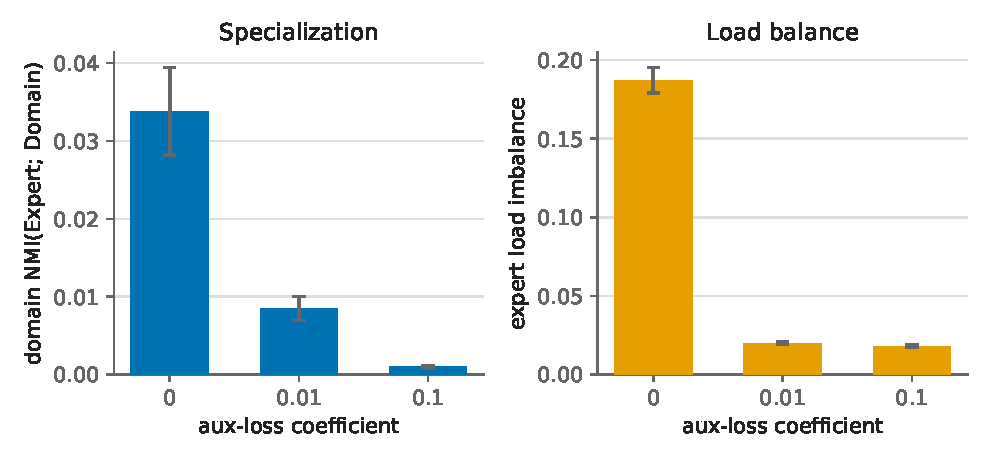
\includegraphics[width=0.85\linewidth]{fig4_auxloss.pdf}
\caption{Domain specialization (left) and expert load imbalance (right) vs.\ the auxiliary
load-balancing coefficient (4 seeds, $\pm1$ std). Both fall monotonically as balancing strengthens.}
\label{fig:f2}
\end{figure}

\paragraph{Shared expert enables specialization.} With balancing off, routed domain-NMI is higher
\emph{with} the shared expert (0.034) than without (0.015, $p=0.029$): the shared expert acts as a
common-capability backstop, consistent with the DeepSeekMoE intuition.

\paragraph{Three retracted findings.} (a) At 3 seeds, removing the shared expert appeared to sharpen
routed specialization; at 4 seeds this collapsed ($p=0.54$) and, once balancing is off, the sign
reverses. (b) We hypothesized the shared monopoly was a \emph{pathology}; a per-token shared-branch
dropout breaks the monopoly entirely (shared share $\rightarrow 0.01$) but yields no perplexity gain
and no specialization gain---consistent with Section~\ref{sec:mech}'s conclusion that the
shared/routed split is a near-neutral reparametrization. (c) We previously reported a
\textbf{non-monotonic dependence on the number of experts}, with a ``Goldilocks'' optimum at
$E{=}8$ and monotonically improving perplexity in $E$. Both halves were confounded: that sweep held
per-expert width fixed, so total routed capacity \emph{and} total parameters grew with $E$ while
the width ratio stayed at 1.0 throughout---which is exactly why all four points fall inside the
single narrow band (0.47--0.56) that Section~\ref{sec:scope} attributes to ratio 1.0, the apparent
optimum lying within that band's residual spread. The perplexity gain ($3.28\rightarrow2.90$) was a
parameter-count effect: at matched parameters perplexity is flat (2.99--3.02). We retract the
non-monotonic law and the ``pick $E$ for engagement'' recommendation that followed from it. We
report all three as negatives.

\paragraph{Distillation (preliminary).} On-the-fly distillation from a Mistral-7B teacher, compared
to a batch/step-matched from-scratch control at 98M tokens, appears to engage the routed branch more
(remove-routed $+1.03\rightarrow+1.74$) but at a small next-token PPL cost and from a single seed;
not established.

\section{Practical recommendations}

\begin{enumerate}
  \item \textbf{Do not diagnose expert redundancy on an undertrained model.} Below a few hundred
  million tokens the shared expert dominates for optimization reasons, not architectural ones;
  measure branch importance as a trajectory, not at a single early checkpoint.
  \item \textbf{To engage the routed experts sooner, slow the shared expert} (e.g.\ a $\times0.3$ LR
  multiplier). This reallocates computation to the routed branch at no measured perplexity
  cost---valuable when routed experts are the object of study or when balanced load is desired. The
  handicap need only cover the early race: ramping the multiplier back to $\times1.0$ by
  $\sim$300M tokens left the reallocation in place through 1B.
  \item \textbf{Set the routed:shared width ratio, not the expert count, to control engagement.}
  How much of the feed-forward computation the routed branch ends up carrying is governed by
  $I/I_{\mathrm{shared}}$: widening the shared expert starves the routed branch even when the routed
  branch is untouched, and narrowing it does the reverse. If you want routed experts that are
  actually used, do not make the shared expert wide. Expert count is close to a free parameter for
  this purpose---it moved neither the split (at matched ratio) nor perplexity (at matched
  parameters) in our sweeps.
  \item \textbf{Report seeds, use matched batch sizes, and match capacity when sweeping
  architecture.} The sign of a specialization effect and the magnitude of branch-importance metrics
  were sensitive to seed and batch size at fixed tokens; and our own \#experts sweep (retraction
  (c)) was confounded because it let total capacity ride along with the variable under study.
\end{enumerate}

\section{Limitations}

Pilot scale (58M--251M parameters, $\leq$1B tokens, 512 context, a single hardware configuration and
data mix). Held-out evaluation uses a skip-offset of the training streams rather than a fully
disjoint split. Held-out NMI and branch-importance magnitudes are sensitive to batch size at fixed
token count, so cross-experiment magnitude comparisons should use matched batches; the
within-experiment, matched-batch comparisons and the token trajectories are the reliable ones. The
width-ratio result of Section~\ref{sec:scope} spans $8\times$ in ratio but at a single depth and a
single token budget, and we characterize the ordering, not a functional form: whether the split
depends on the ratio alone or on ratio and depth jointly is untested. The hysteresis result is
single-seed, at one ramp endpoint and one depth. Distillation results are single-seed. Whether the
$\sim$300M-token crossover and the gradient-race control persist at larger scale is untested.

\section{Conclusion}

In small shared-expert MoEs, the routed experts are not redundant---they are out-competed by the
shared expert in a gradient-exposure race that resolves with training and that a single learning-rate
knob controls at no quality cost, even when applied only temporarily. Where the two branches finally
settle is set by their width ratio rather than by the number of experts, and across a 0.25-to-0.81
range of splits perplexity moves by less than 0.1---the placement of feed-forward computation in a
small MoE is close to a free design choice. The practical takeaways are concrete: do not diagnose
expert redundancy on an undertrained MoE; to engage the routed experts sooner, slow the shared
expert; and to engage them \emph{more}, do not make the shared expert wide. The
methodology---a cheap, controllable, domain-labelled testbed with causal branch
ablation, seed replication, and the willingness to retract---is offered alongside the findings. All
code, configs, and the analysis toolkit run on a single GPU and are released with the paper.

\bibliographystyle{plainnat}
\bibliography{references}

\end{document}
